\documentclass[final]{beamer}
  \mode<presentation>
  {
% you can chose your theme here:
\usetheme{ssc2014}
% further beamerposter themes are available at 
% http://www-i6.informatik.rwth-aachen.de/~dreuw/latexbeamerposter.php
}
  \usepackage{type1cm}
  \usepackage{calc} 
  \usepackage{times}
  \usepackage{wrapfig}
  \usepackage{amsmath,amsthm, amssymb, latexsym}
  \boldmath
  \usepackage[english]{babel}
  \usepackage[latin1]{inputenc}
  \usepackage[orientation=landscape,width=71, height=35,debug]{beamerposter}
  \title{SSC 2014 Case Study Competition}
  \author{Sahir Bhatnagar, Kevin McGregor and Maxime Turgeon}
  \institute{Department of Epidemiology, Biostatistics and Occupational Health, McGill University} 
  \date{May 26, 2013}
  
\usepackage{environ}% Required for \NewEnviron, i.e. to read the whole body of the environment
\makeatletter

\newcounter{acolumn}%  Number of current column
\newlength{\acolumnmaxheight}%   Maximum column height


% `column` replacement to measure height
\newenvironment{@acolumn}[1]{%
    \stepcounter{acolumn}%
    \begin{lrbox}{\@tempboxa}%
    \begin{minipage}{#1}%
}{%
    \end{minipage}
    \end{lrbox}
    \@tempdimc=\dimexpr\ht\@tempboxa+\dp\@tempboxa\relax
    % Save height of this column:
    \expandafter\xdef\csname acolumn@height@\roman{acolumn}\endcsname{\the\@tempdimc}%
    % Save maximum height
    \ifdim\@tempdimc>\acolumnmaxheight
        \global\acolumnmaxheight=\@tempdimc
    \fi
}

% `column` wrapper which sets the height beforehand
\newenvironment{@@acolumn}[1]{%
    \stepcounter{acolumn}%
    % The \autoheight macro contains a \vspace macro with the maximum height minus the natural column height
    \edef\autoheight{\noexpand\vspace*{\dimexpr\acolumnmaxheight-\csname acolumn@height@\roman{acolumn}\endcsname\relax}}%
    % Call original `column`:
    \orig@column{#1}%
}{%
    \endorig@column
}

% Save orignal `column` environment away
\let\orig@column\column
\let\endorig@column\endcolumn

% `columns` variant with automatic height adjustment
\NewEnviron{acolumns}[1][]{%
    % Init vars:
    \setcounter{acolumn}{0}%
    \setlength{\acolumnmaxheight}{0pt}%
    \def\autoheight{\vspace*{0pt}}%
    % Set `column` environment to special measuring environment
    \let\column\@acolumn
    \let\endcolumn\end@acolumn
    \BODY% measure heights
    % Reset counter for second processing round
    \setcounter{acolumn}{0}%
    % Set `column` environment to wrapper
    \let\column\@@acolumn
    \let\endcolumn\end@@acolumn
    % Finally process columns now for real
    \begin{columns}[#1]%
        \BODY
    \end{columns}%
}
\makeatother

%\newlength{\myheight}

\begin{document}
  \begin{frame} 
    \vfill
    
        \begin{acolumns}[t]
          \begin{column}{.32\linewidth}
          
            \begin{block}{Abstract}
    			We consider the effect of economy on the amount of time citizens reported watching television on the ATUS  between 2003 and 2012. Measures of economic performance include GDP, unemployment rate, and stock indices, as reported by federal agencies, with PCA being used to derive an aggregate measure. Using penalized regression methods, we determine the strongest sociodemographic factors (e.g. race, sex, education level, income) influencing television viewing. A hierarchical model is used to allow the association with covariates to vary smoothly with time. To account for the large number of respondents reporting no hours of television viewing, a separate logistic model is proposed.
              \autoheight 
            \end{block}
            
          
          \end{column}
          
          \begin{column}{.32\linewidth}
            \begin{block}{Introduction}
              \begin{itemize}
              	\item Since 2003, the ATUS has been collecting information on how Americans spend a day, what kind of activities they perform, and for how long.
              	\item Over a decade, some 135,000 respondents were asked to walk an interviewer through a selected day.
              	\item The dataset itself contains socio-demographic information about the respondents (e.g. sex, race, income), as well as time-use variables (e.g. sleeping, working, watching TV)
              \end{itemize}
              \autoheight 
            \end{block}
    
          \end{column}
          
          \begin{column}{.32\linewidth}
           \begin{block}{Main questions}
            
            \begin{itemize}
            	\item What effect does the economy have on the amount of time spent watching TV? Does this vary by gender? Does this vary according to your labour force participation? Does this vary across income?

            	\item What are the strongest socio-demographic predictors of time spent watching TV?
            \end{itemize}
            \autoheight
           \end{block}
              
          \end{column}
          
        \end{acolumns}
    
    
    \vfill 
    
    \begin{acolumns}[t]
              \begin{column}{.24\linewidth}
              
                \begin{block}{Main challenges}
        		  \begin{itemize}
        		  	\item About 20\% of respondents reported no TV watching; two separate models are used to address this issue
        		  	
        		  	\item How can economy be measured. \textbf{Note}: economy cannot have a direct, causal effect on TV watching
        		  	
        		  	\item How can we separate the effect of time from the effect of economy
        		  	
        		  	\item How to take into account the stratified sampling scheme
        		  \end{itemize}
        			
                  \autoheight 
                \end{block}
                
              
              \end{column}
              
              \begin{column}{.24\linewidth}
                \begin{block}{Economy}
                	
                  \begin{wrapfigure}{l}{0.5\textwidth}
                  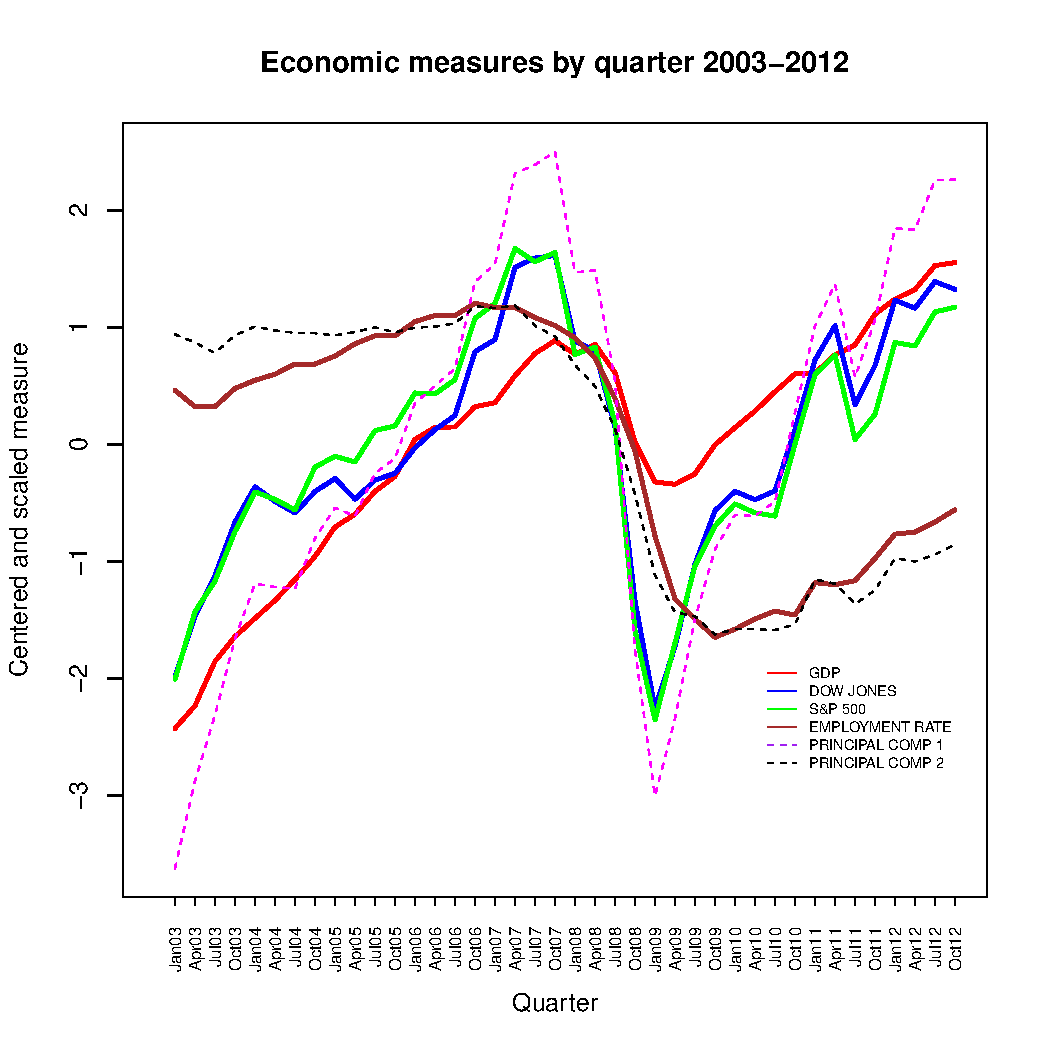
\includegraphics[height=4.5in]{econ_measures.pdf}
                  \end{wrapfigure}
                  Several economic measures were collected via US federal agencies, and an aggregate measurement was constructed using Principal Component Analysis
                  
                  \vspace{2in}
                  \autoheight 
                \end{block}
        
              \end{column}
              
              \begin{column}{.24\linewidth}
               \begin{block}{Stratification}
                \begin{center}
                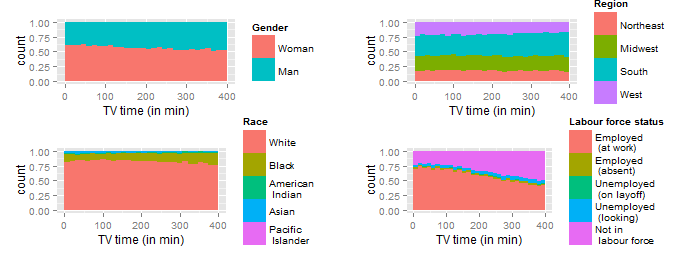
\includegraphics{stratification}
                \end{center}
               
                \autoheight
               \end{block}
               
              \end{column}
               
              \begin{column}{.24\linewidth}
               \begin{block}{Selected socio-demographic variables}
                \begin{itemize}
                	\item Gender, age, region, race, hispanicity, marital status, education level, presence of household children or spouse, US citizenship status,
                	
                	\item Weekly earnings, labour force status, number of jobs, average number of hours worked in a week
                	
                	\item Month and year the interview was conducted, the day of the week, whether it was a holiday
                	
                \end{itemize}
                             
                \autoheight
               \end{block}
                  
              \end{column}
              
            \end{acolumns}
        
        
        \vfill
    
    \begin{acolumns}[t]
    
    \begin{column}{.72\linewidth}
    \begin{center}
   		\LARGE{1. Effect of economy}
    \end{center}
     \begin{block}{Method}
       
       To test for the effect of economy, we use two generalized linear models: gamma regression and logistic regression.
       $$g(\mu_i)=\beta_1ECON1_i+\beta_2ECON2_i + \alpha X_i + \lambda(t_i),$$
       where $X_i$ are the covariates accounting for the stratified sampling scheme (gender, day of the week, region, hispanicity, race) and $\lambda(t)$ is a smooth function of time (measured in months). The smoothing was done via linear extrapolation:
       $$E\left(\lambda(t)|\lambda(t-1),\lambda(t-2),\ldots,\lambda(1)\right) = 2\lambda(t-1) - \lambda(t-2).$$
       The stochastic part of the models are respectively
       $$TVTIME_i\sim \mathrm{Gamma}(\nu, \lambda_i),\hspace{1cm} g(x)=\log(x),\qquad\mbox{and}\qquad TVIND_i\sim \mathrm{Bernouilli}(\pi_i), \hspace{1cm} g(x)=\mathrm{logit}(x).$$
        
     \end{block}
     
     
     \begin{block}{Results}
       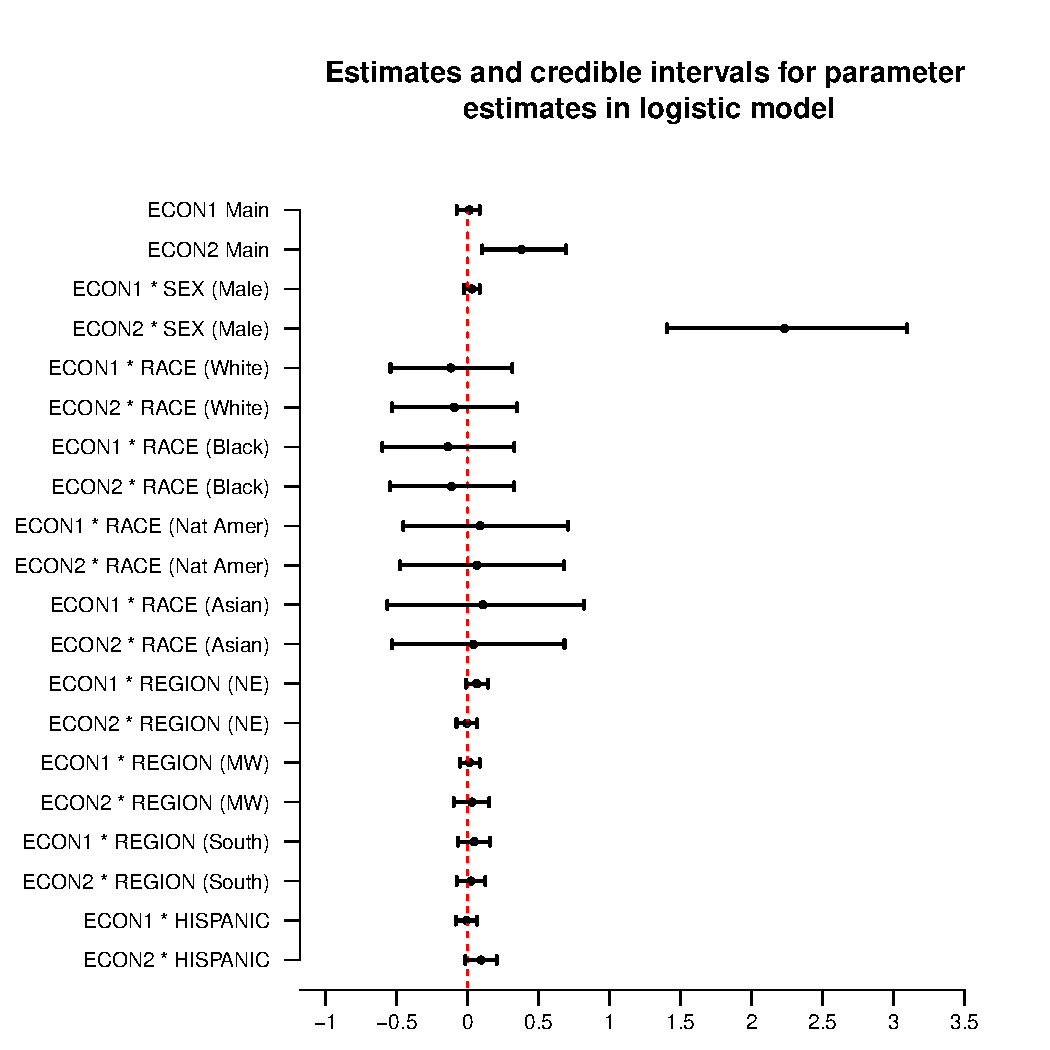
\includegraphics{logit_estimates.pdf}   
       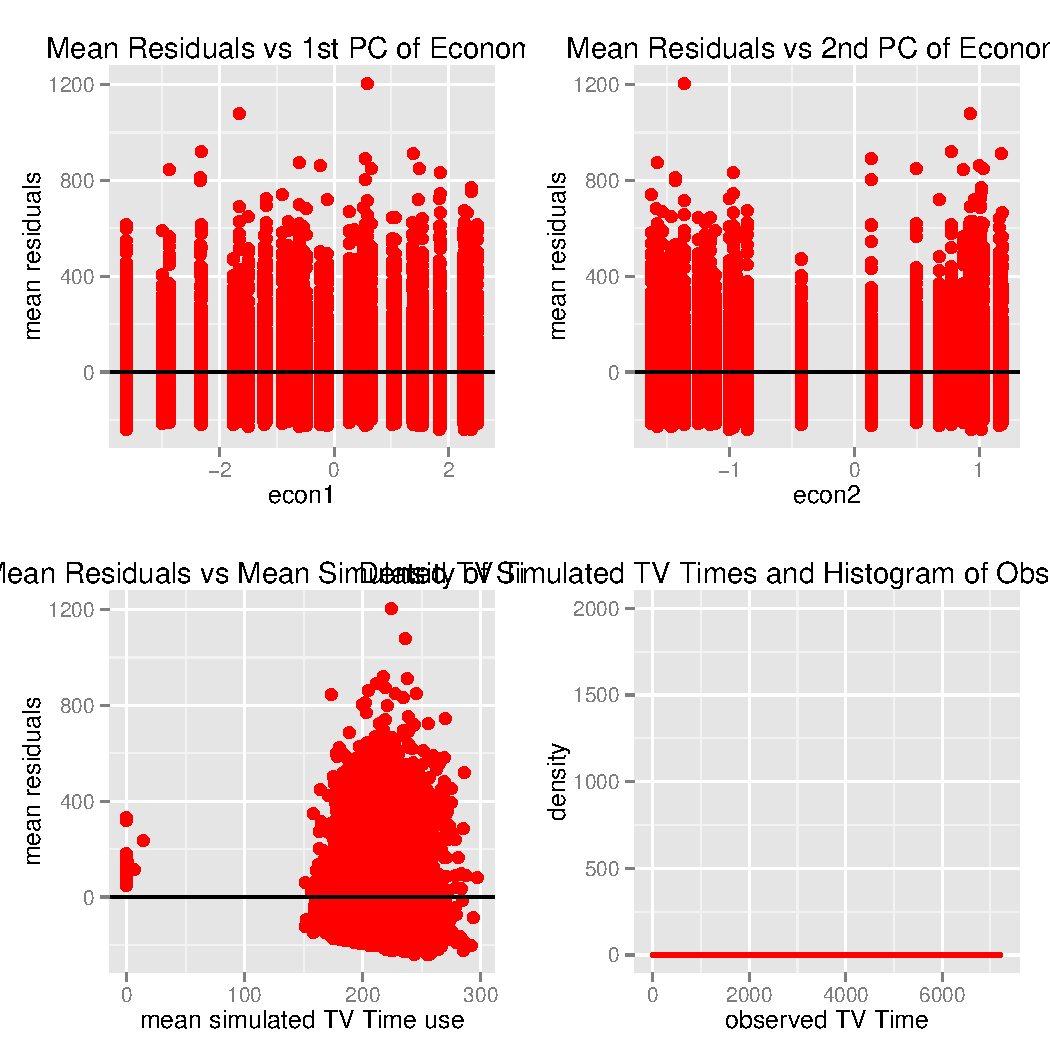
\includegraphics{validation.pdf}
      \autoheight 
     \end{block}
     
                     
    \end{column}
              
    
    \begin{column}{.24\linewidth}
    \begin{center}
    	\LARGE{2. Main socio-demographic predictors}
    \end{center}
     \begin{block}{Method}
     	\begin{itemize}
     		\item We use a penalized generalized linear model to select the most relevant socio-demographic factors. The penalty being used is the group-Lasso penalty (Yuan \& Lin, 2007):
     		$$\lambda \sum_{\ell=1}^{L}\sqrt{p_\ell}\|\beta_\ell\|_2.$$
     		This penalty is used to account for the fact that some predictors are categorical.
     		\item The tuning parameter is selected using 10-fold cross-validation and the one-standard error rule (Hastie \emph{et al.}, \emph{Elements of Statistical Learning})
     	\end{itemize}
        
                     
     \end{block}
          
          
     \begin{block}{Results}
        \begin{itemize}
        	\item For the logistic model, the selected factors are: presence of household children, age, sex, average number of hours worked in a week, and the number of jobs.
        	
        	\item For the gamma model, the selected factors are: presence of household children, age, sex, weekly earnings, presence of spouse in household, average number of hours worked in a week, diary day, education level, race, and the number of jobs.
        \end{itemize}
       \autoheight                   
     \end{block}
     
        
    \end{column}
    
    
    \end{acolumns}
    
    \vfill
    
        \begin{acolumns}[t]
        
        \begin{column}{.24\linewidth}
        		
                 
                 \begin{block}{Discussion}
                 	\begin{itemize}
                 		\item The use of Bayesian techniques provided convenient computations tools. It allowed for both a smooth time effect and exact inference.
                 		\item                  		
                 	\end{itemize}
                  \autoheight   
                 \end{block}
                              
        \end{column}
        
        \begin{column}{.24\linewidth}
		
         
         \begin{block}{Strengths}
         	\begin{itemize}
         		\item The model is effectively separating the economic trend from the time trend
         		\item The measure of economy being used is quite flexible
         		\item The model was able to differentiate between the effect of unemployment and the effect of market behaviour
         	\end{itemize}
          \autoheight   
         \end{block}
                      
        \end{column}
                  
        
        \begin{column}{.24\linewidth}
         
         \begin{block}{Limitations}
         	\begin{itemize}
         		\item The model could be complemented by more model-validation results
         		\item The model does not include the natural auto-regressive structure of the economic variables
         	\end{itemize}
          \autoheight   
         \end{block}
                      
        \end{column}
        
        
         \begin{column}{.24\linewidth}
                 
          \begin{block}{Acknowledgements}
             \begin{center}
             We would like to thank Dr. Celia Greenwood, Dr. Olli Saarela, Dr. Abbas Khalili, and Dr. James Hanley for their help and input on this project.
             \end{center}
             
           \autoheight   
          \end{block}
                              
         \end{column}
        
        
        \end{acolumns}
    
    \vfill 
  \end{frame}
\end{document}
